\documentclass[14pt]{extbook}
\usepackage{multicol, enumerate, enumitem, hyperref, color, soul, setspace, parskip, fancyhdr} %General Packages
\usepackage{amssymb, amsthm, amsmath, bbm, latexsym, units, mathtools} %Math Packages
\everymath{\displaystyle} %All math in Display Style
% Packages with additional options
\usepackage[headsep=0.5cm,headheight=12pt, left=1 in,right= 1 in,top= 1 in,bottom= 1 in]{geometry}
\usepackage[usenames,dvipsnames]{xcolor}
\usepackage{dashrule}  % Package to use the command below to create lines between items
\newcommand{\litem}[1]{\item#1\hspace*{-1cm}\rule{\textwidth}{0.4pt}}
\pagestyle{fancy}
\lhead{Progress Quiz 9}
\chead{}
\rhead{Version B}
\lfoot{8590-6105}
\cfoot{}
\rfoot{Fall 2020}
\begin{document}

\begin{enumerate}
\litem{
Solve the radical equation below. Then, choose the interval(s) that the solution(s) belongs to.\[ \sqrt{8 x - 2} - \sqrt{-3 x + 5} = 0 \]\begin{enumerate}[label=\Alph*.]
\item \( x \in [-0.6,0.03] \)
\item \( x_1 \in [0.2, 0.4] \text{ and } x_2 \in [-0.77,0.78] \)
\item \( \text{All solutions lead to invalid or complex values in the equation.} \)
\item \( x \in [0.6,0.84] \)
\item \( x_1 \in [0.2, 0.4] \text{ and } x_2 \in [1.31,1.82] \)

\end{enumerate} }
\litem{
Solve the radical equation below. Then, choose the interval(s) that the solution(s) belongs to.\[ \sqrt{-48 x^2 + 63} - \sqrt{-2 x} = 0 \]\begin{enumerate}[label=\Alph*.]
\item \( x \in [1.15,1.19] \)
\item \( x_1 \in [1.08, 1.13] \text{ and } x_2 \in [0.17,2.17] \)
\item \( \text{All solutions lead to invalid or complex values in the equation.} \)
\item \( x \in [-1.15,-1.11] \)
\item \( x_1 \in [-1.15, -1.11] \text{ and } x_2 \in [0.17,2.17] \)

\end{enumerate} }
\litem{
Choose the graph of the equation below.\[ f(x) = \sqrt[3]{x + 14} + 4 \]\begin{enumerate}[label=\Alph*.]
\begin{multicols}{2}\item 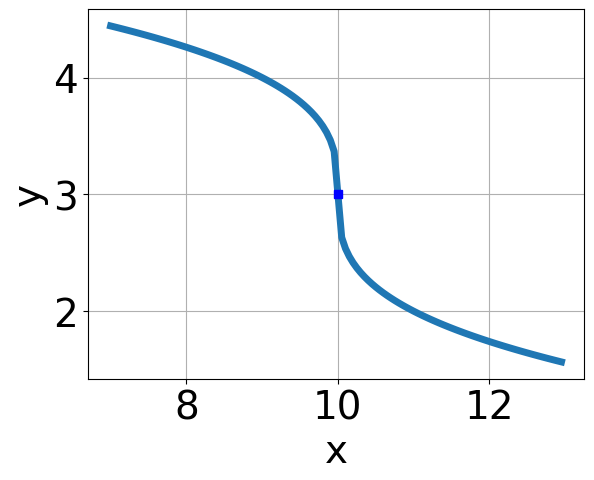
\includegraphics[width = 0.3\textwidth]{../Figures/radicalEquationToGraphAB.png}\item 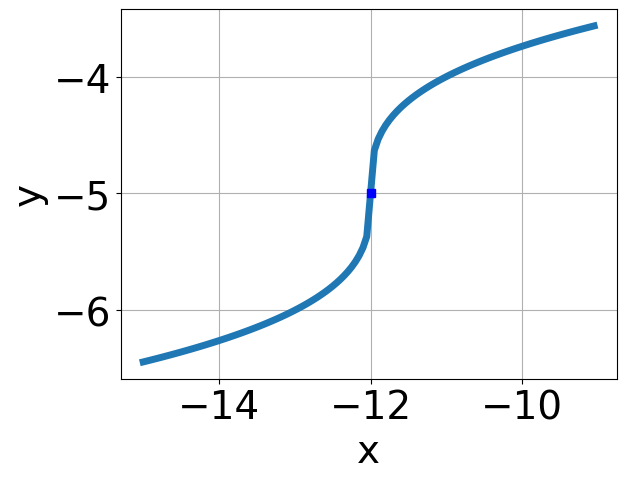
\includegraphics[width = 0.3\textwidth]{../Figures/radicalEquationToGraphBB.png}\item 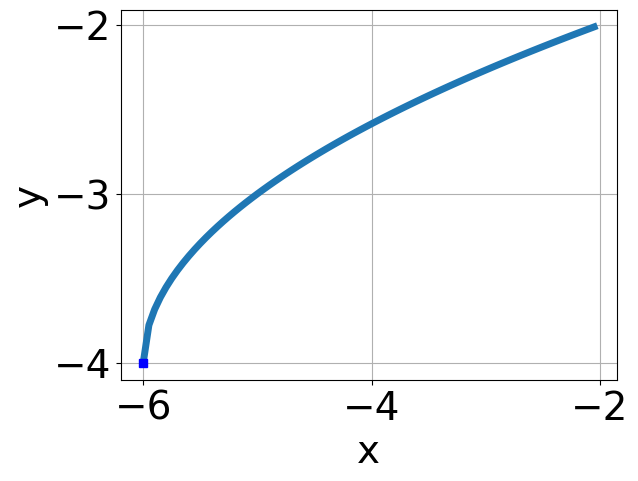
\includegraphics[width = 0.3\textwidth]{../Figures/radicalEquationToGraphCB.png}\item 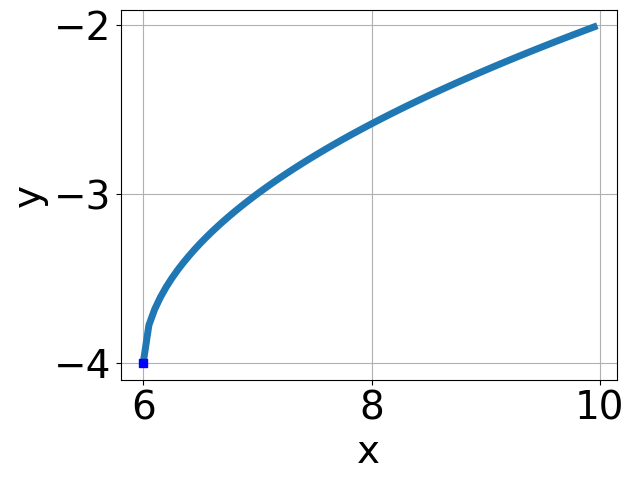
\includegraphics[width = 0.3\textwidth]{../Figures/radicalEquationToGraphDB.png}\end{multicols}\item None of the above.
\end{enumerate} }
\litem{
Choose the equation of the function graphed below.
\begin{center}
    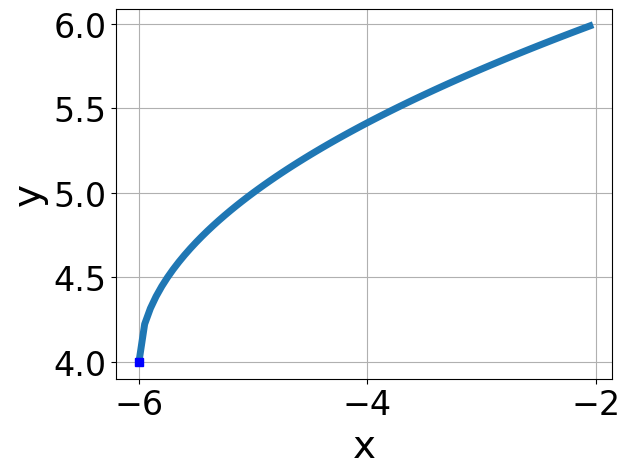
\includegraphics[width=0.5\textwidth]{../Figures/radicalGraphToEquationB.png}
\end{center}
\begin{enumerate}[label=\Alph*.]
\item \( f(x) = - \sqrt{x - 12} - 4 \)
\item \( f(x) = \sqrt{x + 12} - 4 \)
\item \( f(x) = \sqrt{x - 12} - 4 \)
\item \( f(x) = - \sqrt{x + 12} - 4 \)
\item \( \text{None of the above} \)

\end{enumerate} }
\litem{
Choose the equation of the function graphed below.
\begin{center}
    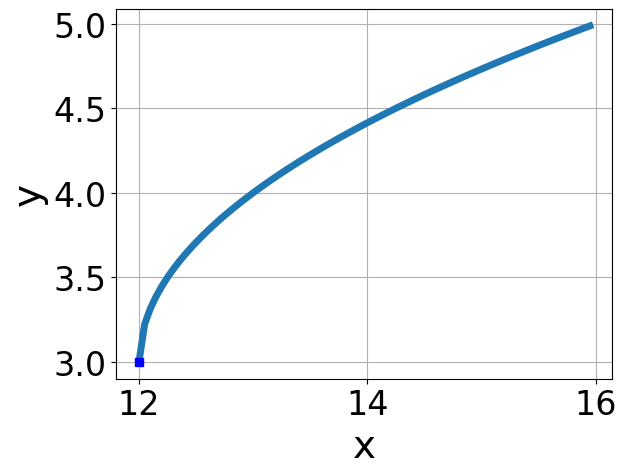
\includegraphics[width=0.5\textwidth]{../Figures/radicalGraphToEquationCopyB.png}
\end{center}
\begin{enumerate}[label=\Alph*.]
\item \( f(x) = \sqrt{x - 14} + 3 \)
\item \( f(x) = \sqrt{x + 14} + 3 \)
\item \( f(x) = - \sqrt{x + 14} + 3 \)
\item \( f(x) = - \sqrt{x - 14} + 3 \)
\item \( \text{None of the above} \)

\end{enumerate} }
\litem{
Solve the radical equation below. Then, choose the interval(s) that the solution(s) belongs to.\[ \sqrt{7 x - 8} - \sqrt{8 x - 2} = 0 \]\begin{enumerate}[label=\Alph*.]
\item \( x \in [-12,-9] \)
\item \( x \in [-6,-1] \)
\item \( \text{All solutions lead to invalid or complex values in the equation.} \)
\item \( x_1 \in [-1.75, 2.25] \text{ and } x_2 \in [0.14,6.14] \)
\item \( x_1 \in [-6, -1] \text{ and } x_2 \in [0.14,6.14] \)

\end{enumerate} }
\litem{
What is the domain of the function below?\[ f(x) = \sqrt[8]{-8 x - 4} \]\begin{enumerate}[label=\Alph*.]
\item \( [a, \infty), \text{where } a \in [-3, -1] \)
\item \( (-\infty, a], \text{where } a \in [-3.05, -1] \)
\item \( (-\infty, \infty) \)
\item \( (-\infty, a], \text{ where } a \in [-1.55, 0.9] \)
\item \( [a, \infty), \text{where } a \in [-1.5, 4.5] \)

\end{enumerate} }
\litem{
What is the domain of the function below?\[ f(x) = \sqrt[5]{7 x - 8} \]\begin{enumerate}[label=\Alph*.]
\item \( \text{The domain is } [a, \infty), \text{   where } a \in [1.13, 1.26] \)
\item \( \text{The domain is } (-\infty, a], \text{   where } a \in [0.9, 3] \)
\item \( \text{The domain is } (-\infty, a], \text{   where } a \in [0.8, 1] \)
\item \( \text{The domain is } [a, \infty), \text{   where } a \in [0.62, 1.06] \)
\item \( (-\infty, \infty) \)

\end{enumerate} }
\litem{
Solve the radical equation below. Then, choose the interval(s) that the solution(s) belongs to.\[ \sqrt{-12 x^2 - 48} - \sqrt{50 x} = 0 \]\begin{enumerate}[label=\Alph*.]
\item \( x \in [-3.4,-2.1] \)
\item \( x_1 \in [1.75, 3.35] \text{ and } x_2 \in [-1,2.4] \)
\item \( x_1 \in [-3.4, -2.1] \text{ and } x_2 \in [-2,0.9] \)
\item \( x \in [-2.12,-1.09] \)
\item \( \text{All solutions lead to invalid or complex values in the equation.} \)

\end{enumerate} }
\litem{
Choose the graph of the equation below.\[ f(x) = \sqrt[3]{x - 12} + 6 \]\begin{enumerate}[label=\Alph*.]
\begin{multicols}{2}\item 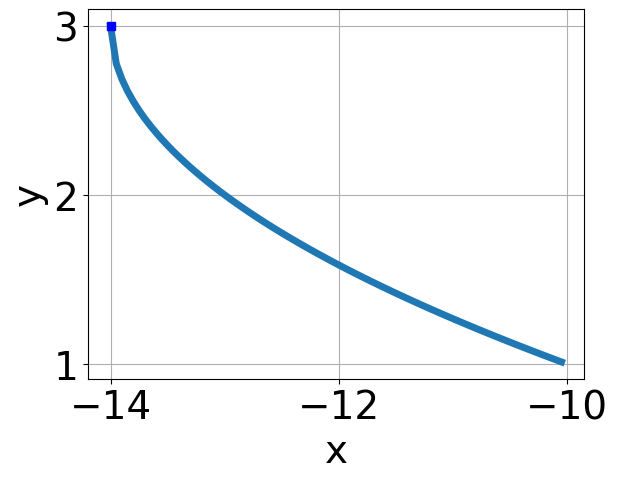
\includegraphics[width = 0.3\textwidth]{../Figures/radicalEquationToGraphCopyAB.png}\item 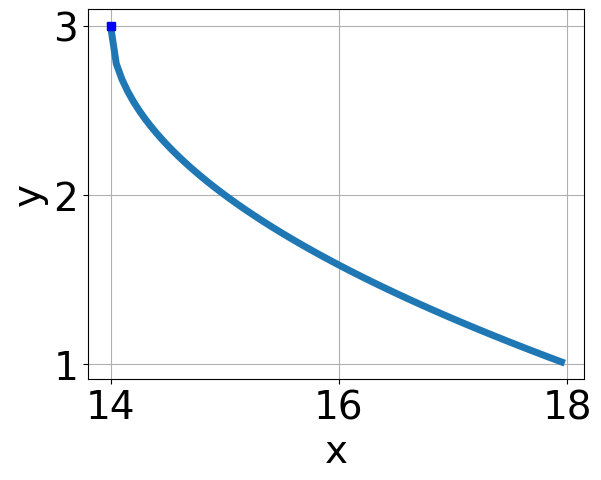
\includegraphics[width = 0.3\textwidth]{../Figures/radicalEquationToGraphCopyBB.png}\item 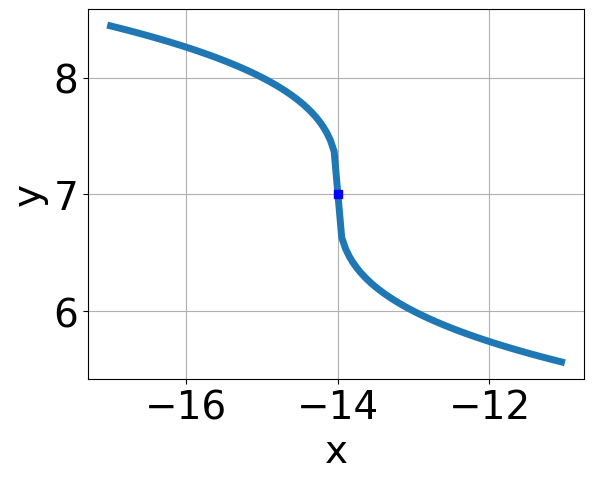
\includegraphics[width = 0.3\textwidth]{../Figures/radicalEquationToGraphCopyCB.png}\item 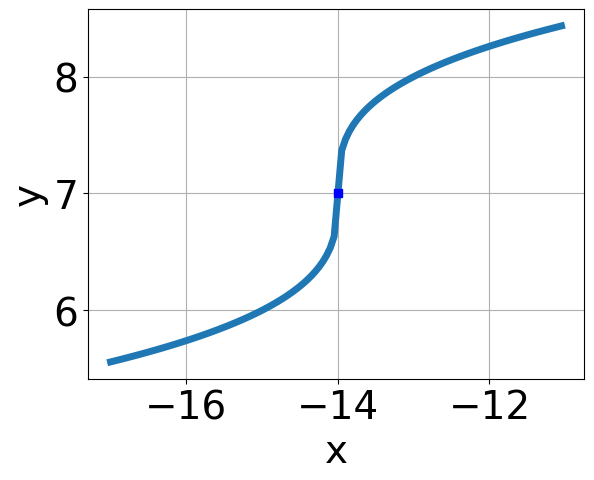
\includegraphics[width = 0.3\textwidth]{../Figures/radicalEquationToGraphCopyDB.png}\end{multicols}\item None of the above.
\end{enumerate} }
\end{enumerate}

\end{document}